\begin{flushleft}
Per fare il confronto abbiamo scritto lo script:
\lstinputlisting[language=matlab]{cap_4/es10/es10.m}
Il ciclo annidato a linea 15 calcola $y = \sum_{k=0}^{m} (a_k\cdot x^k)$ che trova i valori dipendenti dalle ascisse, il ciclo a linea 9 calcola i valori di $y$ indipendenti. Il confronto tra le due rette è il seguente:
\begin{figure}[H]
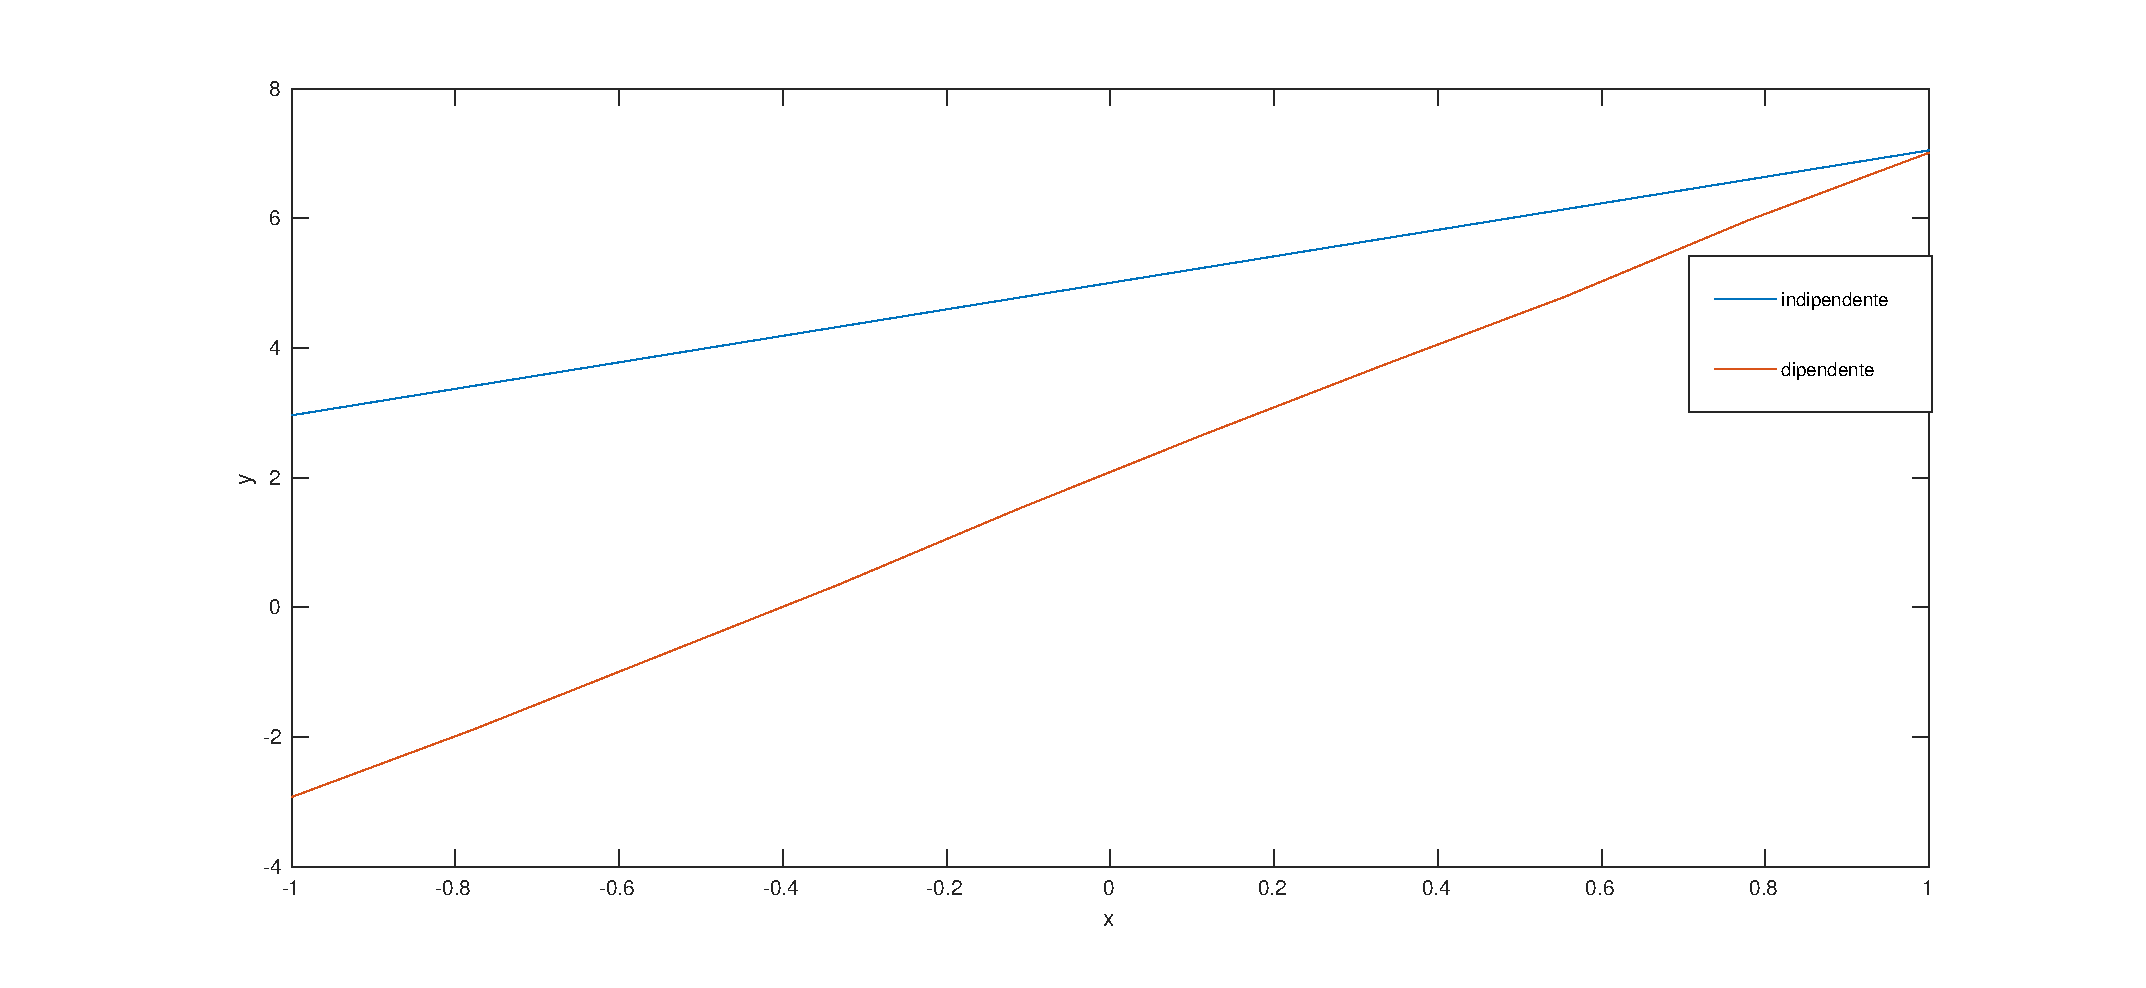
\includegraphics[width=480px, height=280px]{plot/fes410}
\caption{\texttt{Confronto tra y dipendente e indipendente}}
\end{figure}
\end{flushleft}